\chapter{序論} % 章のタイトル

% \includegraphics[width=??cm]{hoge.eps} % 図(EPS形式)を読み込む場合

\section{背景} % sectionのタイトル

% 以下に背景,関連する環境状況,技術に関する概要を記述.

近年,インターネット技術やセンサー技術の進化を背景に,パソコンやスマートフォンなどのインターネット端末に加え,家電や自動車などの様々なものに通信機能を搭載したIoTデバイスが普及し始めている.総務省によると政界中のIoTデバイスの数は図\ref{fig:IoT}のように2017年時点でIoTデバイスが約275億台存在し,2020年にはIoTデバイスが403億台に及ぶと予想されている\cite{IoT}.
 \begin{figure}[hb]
 \centering
    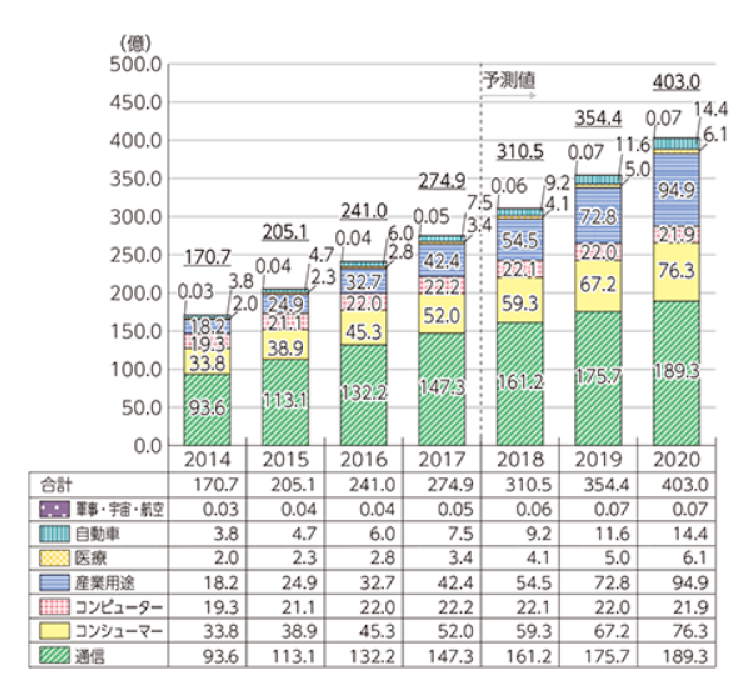
\includegraphics{figures/IoT_device.eps}
    \caption{世界のIoTデバイス数の推移及び予測}
 \label{fig:IoT}
 \end{figure}
 \clearpage
%参考文献を入れ直す
%タイトルに"(~~より引用)"を付け加える.

IoTデバイスの普及に伴い,IoTデバイスを対象としたマルウェアが急増している.
IoTデバイスの重要な問題の1つとしてセキュリティ問題が挙げられる.IoTデバイスのユーザ名やパスワードを初期設定の状態で使用する場合が多いことやデバイスの資源が限られていることから,セキュリティが十分に考慮されていない事がある.そのため,IoTデバイスを対象としたマルウェアが脅威となっている.その中でもネットワークサービスを停止させる深刻な問題を引き起こしているマルウェアにはDDoS(Distributed Denial of Service)攻撃を行っているものが多く存在し,その対策が重要視されている.DDoS攻撃は,攻撃者が複数の他人のコンピュータを利用し,公開されているサービスに大量のデータを送りつける事によって処理負荷を与えサービスを機能停止に追い込む攻撃である.代表的なDDoS攻撃を行うマルウェアとしてMiraiが挙げられる.Miraiを利用して2016年10月に発生した,DNSサーバープロバイダであるDyn社へのDDoS攻撃ではIoTデバイスによるボットネットが利用され史上最大規模である620Gbpsの攻撃が観測された\cite{Dyn}.その後,Miraiのソースコードが公開され,Owari,Satori,OkiruといったMiraiの亜種の開発が盛んに行われるようになった.2017年には,Windows PCを踏み台にして感染可能なIoTデバイスを探索するMiraiが観測された\cite{newMirai}.このMiraiはDoS攻撃を行う機能を有していないが,探索後にログイン可能な端末がLinuxデバイスであればDoS攻撃機能を有したMiraiをダウンロードさせ,Windows PCであればスキャン機能に特化したMiraiをダウンロードさせ,さらなるMiraiを様々なIoTデバイス拡散することが可能になっている.MiraiやMirai亜種のマルウェアによって,多くのIoTデバイスがDDoS攻撃に不正利用されるようになったことから,国立研究開発法人情報通信研究機構がパスワード設定などに不備のあるIoT機器の実態把握を目的として日本国内のIPv4アドレスを対象にSSH,Telnet,HTTPであるTCPの22番,23番,80番ポートを対象にポートスキャンを行った\cite{国立}.IoTデバイスの不正利用によるDDoS攻撃が問題視されており,社会的に注目されている.

\section{IoTデバイスで検知を行う必要性}

IDS(Instrusion Detection System)と呼ばれるマルウェアによる不正な通信やホストへの侵入,ファイルの改ざん等の不正な挙動の兆候を検出するシステムの設置場所としてネットワーク上に設置するネットワーク型と端末上に設置するホスト型の2種類が考えられる.ネットワーク型のIDSでは,ネットワークに流れるデータを取得して解析し,異常がないか確認する.不正が疑わ得れるデータを検知したときには管理者に知らせる.ネットワーク上でネットワークトラフィックからDDoS攻撃を判別するのは難しく誤検知する可能性が考えられる.しかし,マルウェアに基づいて作成されたデータを用いたパターンマッチングによる検知手法では,誤検知率が低く既存のマルウェアを確実に検知できる利点が有る.公開されているソースコードを基に作成されたマルウェアは,オリジナルのマルウェアと共通するシグネチャが存在すると考えられるためパターンマッチングによる検知で亜種のマルウェアにも対応できると想定される.脅威となっているマルウェアは,十分に管理が行われていないIoTデバイスで散見される,放置された初期パスワードのままのアカウントや,保守されていないシステムの脆弱性をついた攻撃を行うため,侵入されてしまうことは前提とすべきである.そのため,デバイスの性能が限られているIoTデバイス上でもマルウェアの検知を行う必要がある.

\section{マルウェアMiraiの概要}

Mirai\cite{Mirai}は,ネットワーク上で公開されているLinuxで動作するデバイスを不正利用し,DDoS攻撃を行うマルウェアである.ネットワークカメラやルータといったIoTデバイスをターゲットにしている.ソースコードはgithub\cite{code}上で公開されており,誰でも使用可能である.Miraiは,C\&Cサーバー,MySQL,Loader,botの4つから構成される.Miraiの概要を図\ref{fig:Mirai_system}に示す.

\begin{figure}[h]
   \centering
      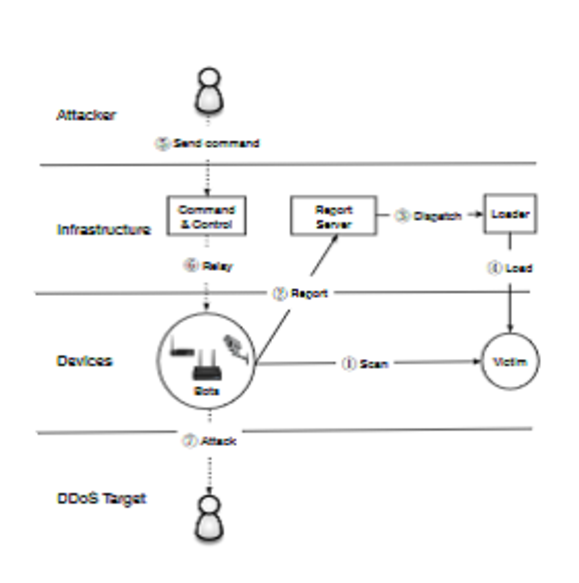
\includegraphics[width=100mm]{figures/s.eps}
      \caption{Miraiの概要図}
   \label{fig:Mirai_system}   
\end{figure}
%新しいものを入れる.

C\&Cサーバーは,ボットやユーザーからの接続されるのを待機しており,主な機能としてボット管理機能,ユーザー管理機能,攻撃指示機能がある.MySQLにはユーザーのリストと攻撃履歴が記録されるようになっている.botは,C\&Cサーバーからのコマンドを待機し,感染先でボットネットに加えられる新しいデバイスを探索するスキャン活動を行う.スキャン活動を行いログインできる端末を見つけた場合には,IPアドレス,ポート,ログイン情報をスキャンサーバーへと送る.感染経路について,Miraiは、Telnetログインが可能な場合に感染する.Loaderは,スキャン活動からレポートサーバーに送られた攻撃対象の情報をもとにTelnetログインを試みる.Telnetログインに成功した際には,攻撃者が用意したhttpサーバーまたはtftpサーバーから,Miraiのバイナリファイルを対象のIoTデバイスにダウンロードしbotを実行させる.botの動作後には,C\&Cサーバーとの通信を始め,C\&Cサーバーから送られてくる攻撃命令を受け取り,IoTデバイスが特定のサーバーに攻撃を始める
.C\&CサーバーによるDDoS攻撃命令は表\ref{tab:attack}のように10種類存在している.

\begin{table}[h]
   \caption{攻撃種類}
   \centering
   \label{tab:attack}
   \begin{tabular}{|l|l|}
   \hline
   攻撃種類                            & 詳細 \\ \hline \hline
   UDP攻撃                           &   UDPパケットを大量に送信する \\ \hline
   プレーンUDP攻撃                    & 高速化のために最適化を行いUDPパケットを大量に送信する   \\ \hline
   SYN攻撃                           &  SYNパケットを大量に送信する  \\ \hline
   ACK攻撃                           &  ACKパケットを大量に送信する  \\ \hline
   HTTP攻撃                          &  HTTPリクエストを大量におくる  \\ \hline
   DNSリゾルバ攻撃                       &  DNSサーバーへ大量の名前解決のためのリクエストを送信する  \\ \hline
   GRE IP 攻撃                       &  GREプロトコルによるパケットを大量に送信する  \\ \hline
   GREイーサネット攻撃                     &  イーサネットとGREプロトコルによるパケットを大量に送信する  \\ \hline
   VSE攻撃                           &  ゲームエンジンに対してUDPパケットを大量に送信する  \\ \hline
   STOMP攻撃                         &  TCPセッション確立後にACKパケットを大量に送信する  \\ \hline
   \end{tabular}
\end{table}


\section{研究目的}
本研究では,IoTデバイス上でDDoS攻撃を行うマルウェアMiraiとその亜種の未知のマルウェア検知である.マルウェアだと疑われるバイナリファイルからシンボルテーブルと呼ばれる使用されている関数名,変数名を取得し,マルウェアが持つ独自の関数を持っていた場合に,マルウェアだと検出する.しかし,stripと呼ばれるバイナリファイルのシンボルテーブルを削除するコマンドなどの検知対策が行われた場合には,検知が行えない.マルウェアによって呼び出される内部関数によって呼び出されるシステムコール系列を用いた検知を行う事によって,検知対策がなされた場合でもマルウェアの検出が可能である.
%研究内容がシンプルすぎるのでIoTデバイス上で検知する,亜種の検知ができるとか大事な部分が抜けている.シンボルテーブルの提案手法とシステムコール呼び出し履歴を用いた手法のそれぞれの位置づけと狙いの違いを記述する.

\section{論文の構成}
%書き方がよくわからないので後で確認を行う.
本論文では,6章から構成されている.1章では,本研究の背景や研究目的について述べる.2章では,関連研究とその課題について述べる.3章では,シンボルテーブルを用いた検知手法の提案についてシンボルテーブルを用いたマルウェアの検出方法について述べる..4章では,システムコール呼び出し履歴を用いた検知手法について述べ,straceによるマルウェアの検出方法の課題点と解決方法について述べる.5章では,提案システムによるマルウェアの検知精度について述べ,6章でまとめる.